\section{Theorie}
\label{sec:Theorie}

\subsection{Verwendete Naturkonstanten im Überblick}

Die in Tabelle \ref{tab:NatKonst} zusammengestellten Naturkonstanten sind \cite{scipy} entnommen. 
Das Bohr'sche Magneton ist über 
\begin{equation*}
    \symup{\mu}_\text{B}=\frac{\symup{e\hbar}}{2\symup{h}}=\frac{\symup{eh}}{4\symup{h\pi}}
\end{equation*}
definiert.

    \begin{table}
        \centering
        \caption{Für das Protokoll benötigte Naturkonstanten auf einen Blick.}
        \label{tab:NatKonst}
        \begin{tabular}{l c c c}
            \toprule
            Naturkonstante &
            Formelzeichen &
            Wert &
            Einheit \\
            \midrule
            Elementarladung                 & $\symup{e}          $   & $\num{1.602176634e-19}$   & \si{\coulomb} \\
            Planck'sches Wirkungsquantum    & $\symup{h}            $ & $\num{6.62607015e-34}$    & \si{\joule\second} \\
            Boltzmann-Konstante             & $\symup{k}_\text{B}   $ & $\num{1.380649e-23}$      & \si{\joule\per\kelvin} \\
            Magnetische Permeabilität       & $\symup{\mu}_0        $ & $\num{1.2566370614e-06}$  & \si{\newton\per\ampere\squared} \\
            Masse eines Elektrons           & $\symup{m_e}          $ & $\num{9.1093837015e-31}$  & \si{\kilo\gram} \\
            Avogadro-Konstante              & $\symup{N}_\text{A}   $ & $\num{6.02214076e+23}$    & \si{\per\mole} \\
            Bohr'sches Magneton             & $\symup{\mu}_\text{B} $ & $\num{9.2740100784e-24}$  & \si{\joule\per\tesla} \\
            \bottomrule
        \end{tabular}
    \end{table}

\subsection{Berechnung der Suszeptibilität paramagnetischer Stoffe}

    Die magnetische Flussdichte $\vec{B}_0$ im Vakuum ist mit der magnetischen Feldstärke $\vec{H}$ durch ${\vec{B}_0=\symup{\mu}_0 \vec{H}}$
    gegeben. Diese Flussdichte unterscheidet sich von der, wenn ein Material sich im Vakuum befindet. 
    In einem solchen Fall gilt 
    \begin{equation}
        \vec{B}_\text{M}= \vec{B}_0 + \vec{M} \,.
        \label{eqn:Flussdichte}
    \end{equation}
    $\vec{M}$ stellt hierbei die Magnetisierung dar und lässt sich auf das durchschnittliche magnetische Moment der Elementarteilchen 
    zurückführen, welche multipliziert mit der Anzahl pro Volumeneinheit und der magnetischen Feldkonstante eben die Magnetisierung ergeben.
    Eine ebenfalls gültige Formel wird durch 
    \begin{equation*}
        \vec{M}=\symup{\mu}_0 \chi \vec{H}
    \end{equation*}
    ausgedrückt.
    Die Suszeptibilität $\chi$ ist an dieser Stelle die für einen Stoff charakteristische Größe. 

    Bei Diamagneten liegt der Wertebereich zwischen $-1$ und $0$, sie werden aus einem Bereich höherer Feldstärke rausgedrückt, 
    Paramagneten mit einer positiven Suszeptibilität werden hineingezogen. 

    Das atomare magnetische Moment, dessen Mittelung die Magnetisierung definiert, hängt eng mit den Drehimpulsen der einzelnen 
    Elektronen in der Atomhülle zusammen. 
    Der Drehimpuls des Atomkerns kann -- vor allem bei den in diesem Experiment zu untersuchendnen Stoffen -- vernachlässigt 
    werden; ausschlaggebend wird er vor allem dann, wenn ein starkes äußeres Magnetfeld vorhanden ist.

    Somit setzt sich der atomare Gesamtdrehimpuls $\vec{J}$ aus dem Bahndrehimpuls $\vec{L}$ und dem Eigendrehimpuls -- dem 
    Spin -- $\vec{S}$ zusammen:
    \begin{equation*}
        \vec{J}=\vec{S}+\vec{L} \,.
    \end{equation*}
    
    Durch Berücksichtigung der Quantisierung bestimmter Größen lässt sich 
    \begin{equation}   
        \chi = \frac{\symup{\mu}_0 \symup{\mu} _\text{B}^2 g_J^2 NJ(J+1)}{3\symup{k}T}
        \label{eqn:chii}
    \end{equation}
    für die Suszeptibilität herleiten\cite{Versuchsanleitung}. 
    Näherungen werden bei dem gyromagnetischen Verhältnis des freien Elektrons $g_\text{S}$ vorgenommen, welches in den Zwischenrechnungen auftaucht und 
    abgesehen von ein paar Promillen Abweichungen den Wert $2$ annimmt. 
    Ebenfalls lässt sich die sogenannte Brillouin-Funktion nähern, da im Experiment bei Zimmertemperatur und mit 
    Magnetfeldern, die nicht größer als $\SI{1}{\tesla}$ sind, gearbeitet wird.

    Der Landé-Faktor $g_J$ wird an dieser Stelle durch 
    \begin{equation}
        g_J=\frac{3J(J+1)+S(S+1)-L(L+1)}{2J(J+1)}
        \label{eqn:lande}
    \end{equation}
    gegeben, wobei $S$, $L$ und $J$ die Quantenzahlen der bereits genannten Drehimpulse darstellen, die sich aus der Summe
    der Quantenzahlen der an der Magnetisierung beteiligten Elektronen ergeben -- die Drehimpulsquantenzahlen der restlichen, nicht beitragenden
    Elektronen summieren sich gerade zu Null. 

\subsection{Die Hund'schen Regeln und das Pauli-Prinzip hinsichtlich Seltener-Erd-Verbindungen}
\label{sub:wauwau}

    Der Landé-Faktor Seltener-Erd-Verbindungen lässt sich mithilfe der Hund'schen Regeln berechnen. 
    Sie legen fest, welche Quantenzahlen $J$, $L$ und $S$ in Gleichung \eqref{eqn:lande} eingesetzt werden müssen. 

    Seltene Erden haben eine voll besetzte Elektronenhülle bis zur 5p-Schale. Darauf aufbauend befinden sich je nach 
    Element und Ionisationszustand noch zwei 6s-Elektronen und weitere 4f-Elektronen in der Elektronenhülle. 
    Die 4f-Elektronen sind die für die Magnetisierung entscheidenden Teilchen -- sie legen die Quantenzahlen fest, 
    die der anderen Schalen kompensieren sich gegenseitig. 

    Die Hund'schen Regeln sind\cite{Versuchsanleitung}:
    \begin{enumerate}
        \item Der Eigendrehimpuls beziehungsweise der Spin $S$ ist maximal, woraus eine möglichst parallele Orientierung 
            der einzelnen Elektronenspins resultiert.    
        \item Der Bahndrehimpuls $L$ ist maximal, also ebenfalls nach Möglichkeit parallel. 
        \item Wenn eine Unterschale maximal zur Hälfte gefüllt ist, ergibt sich ${J=L-S}$, andernfalls ${J=L+S}$.
    \end{enumerate}
    Wichtig zu wissen ist hierbei: 
    \begin{itemize}
        \item Der Spin $s$ eines einzelnen Elektrons nimmt die Werte $\sfrac{1}{2}$ oder $\sfrac{-1}{2}$ an. 
        \item Hierbei seien die summierten Werte durch $S=\sum_i s_i$ und $L=\sum_i l_i$ gegeben. 
        \item Die ausschlaggebende Unterschale ist 4f; das bedeutet, dass die Hauptquantenzahl ${n=4}$ ist.
        \item Für die Quantenzahlen des Bahndrehimpuls dieser Schale gilt folglich: $|l_i| \in [0,n-1] \Rightarrow l_i \in [-3,3]$ .
    \end{itemize}

    Ein letzter wichtiger Aspekt für die Bestimmung der Quantenzahlen stellt das Pauli-Prinzip dar. 
    Es besagt, dass ein zu einem Elektron gehöriges Triple an Quantenzahlen $(n,l,s)$ nicht doppelt innerhalb eines Elektrons vorkommen darf. 
    Das bedeutet für die 4f-Schale, dass $n=4$ ist und somit $(l,s)$ innerhalb der befindlichen Schale paarweise verschieden sein müssen. 
    
    Mithilfe dieser Gesetzmäßigkeiten können im Nachhinein die Theorie-Werte für die Suszeptibilität der entsprechenden Stoffe bestimmt werden. 

\subsection{Messung der Suszeptibilität}
\label{sub:messmethode}

    Wird eine Spule mit Materie gefüllt, verstärkt sich (bei positiver Suszeptibilität) die magnetische Flussdichte gemäß \eqref{eqn:Flussdichte}. 
    Dadurch vergrößert sich auch die Induktivität $L$ einer langen Spule um den Betrag 
    \begin{equation}
        \Delta L=\symup{\mu}_0 \chi Q \frac{n^2}{l} \,,
    \end{equation}
    wobei $Q$ die Querschnittsfläche des Füllmaterials, $n$ die Windungszahl und $l$ die Länge der Spule  sind. 

    Diese Größe ist für gewöhnlich sehr klein, deshalb muss die Messapparatur präzise Messungen der Induktivität ermöglichen.
    Eine mögliche Messschaltung ist in Abbildung \ref{fig:TolleSchaltung} zu sehen.
    \begin{figure}
        \centering 
        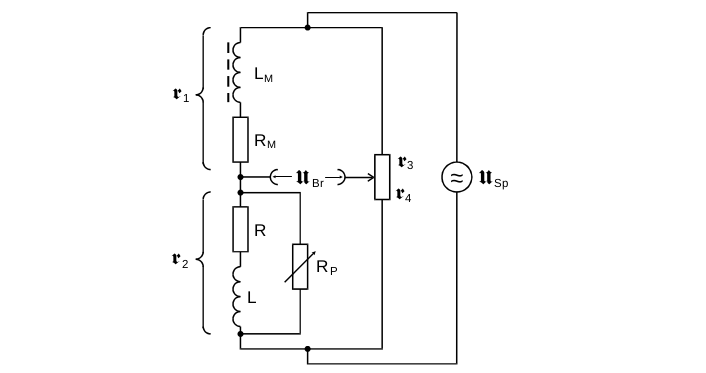
\includegraphics[width=\textwidth]{plots/TolleSchaltung.png}
        \caption{Eine Brückenschaltung zur Bestimmung der Suszeptibilität\cite{Versuchsanleitung}.}
        \label{fig:TolleSchaltung}
    \end{figure}
    Verwendet wird eine sogenannte Brückenschaltung und zwei Spulen, die eine mit der zu untersuchenden Füllung, 
    die andere ohne. 
    Aus der Regulierung der Brückenwiderstände $R_3$ und $R_4$ kann die Brückenspannung $U_\text{Br}$ auf nahezu Null abgeglichen werden. 
    Dies lässt Rückschlüsse auf die verschiedenen Widerstände zu. 

    In diesem Fall führen folgende Annahmnen zur Berechnung der Suszeptibilität:

    Die Verlustwiderstände $R$ und $R_\text{M}$ sind annähernd gleich, da es sich bei den Spulen -- ungeachtet etwaiger 
    Materiefüllungen -- um baugleiche Exemplare handelt. 
    Und eben weil es sich um Verlustwiderstände handelt, sollten sie im Vergleich zu dem Widerstand $R_\text{P}$ gering sein, 
    also $R$ beziehungsweise $R_\text{M}\ll R_\text{P}$. 

    Des Weiteren sei der regelbare Widerstand über das Potentiometer rein ohmsch, das heißt, er bewirkt keine Phasenverschiebung des Stroms
    und die physikalische Größen des Widerstands sind reell. 
    Zudem sei die Annahme, dass $R_3\approx R_4$, da die Spulen wie bereits erwähnt nahezu gleiche Induktivitäten haben 
    ($\Delta L \ll L$) und daher keine große Differenzen bei den Brückenwiderständen zu erwarten sind. 

    Die Feststellung, dass $\Delta L \ll L$, wird ebenfalls zur Herleitung der Formel verwendet. 

    Unter der Annahme, dass die Frequenz hinreichend groß ist, sodass $\omega^2L^2\gg R^2$ gilt, lässt sich die Suszeptibilität
    zu 
    \begin{equation}
        \chi =4\frac{F}{Q}\frac{U_\text{Br}}{U_\text{Sp}}
        \label{eqn:hatschi}
    \end{equation}
    mit der Querschnittsfläche $F$ der Spule und der Speisespannung $U_\text{Sp}$ bestimmen\cite{Versuchsanleitung}.

    Ein weiterer Ausdruck für die Suszeptibilität ohne Verwendung der angelegten Spannungen ergibt sich aus der 
    sogenannten Abgleichbedingung  der Brückenschaltung. Auch wird wieder die Annahme $\Delta L \ll L$ benutzt. 
    Zusätzlich wird noch die Größe $\Delta R$ mit 
    \begin{equation*}
        R'_3=R_3 +\Delta R
    \end{equation*}
    definiert, die die Änderung des Widerstands $R_3$ bei Einführen von Materie in die eine Spule quantisiert.
    Dementsprechend gilt 
    \begin{equation*}
        R'_4=R_4-\Delta R \approx R_3 - \Delta R\,.
    \end{equation*}
    Daraus ergibt sich die Gleichung\cite{Versuchsanleitung}
    \begin{equation}
        \chi = 2 \frac{\Delta R \cdot F}{R_3 \cdot Q}\,.
        \label{eqn:chii2}
    \end{equation}

\subsection{Eliminieren der Störspannungen}

    An den Ausgängen der Brückenschaltung werden nicht vermeidbare Störspannungen gemessen, die die geringen Signalspannungen 
    der in Kapitel \ref{sub:messmethode} beschriebenen Messungen vollkommen überlagern würden. 
    Eine Möglichkeit besteht dennoch bei Verwendung eines sogenannten Selektivverstärkers, der bei einer bestimmten Frequenz $\nu _0$
    die Eingangsspannung $U_\text{E}$ unverfälscht als Ausgangsspannung $U_\text{A}$ durchlässt. 
    Er kann also zur Unterdrückung von Spannungen mit unerwünschter Frequenz verwendet werden. 
    Darin liegt der Nutzen für diese Messung: 
    Die Signalspannungen haben nur eine Frequenz, nämlich die der Speisespannung, wohingegen die Störspannungen sich -- 
    vermutlich kontinuierlich -- über ein ganzes Spektrum erstrecken. 
    Mithilfe des Selektivverstärkers können also alle Störspannungen weitestgehend herausgefiltert werden, die nicht die 
    bewusste Durchlassfrequenz $\nu _0$ haben -- diese lassen sich leider mit dieser Methode nicht eliminieren. 

    Eine wichtige Kenngröße eines Selektivverstärkers ist hierbei die sogenannte Güte $Q$ -- nicht zu verwechseln mit der 
    Querschnittsfläche $Q$ des Füllmaterials. 
    Sie gibt das Verhältnis der Breite der Gaußkurve zur Durchlassfrequenz an, also mit Blick auf Abbildung \ref{fig:Kaffeefilter}
    \begin{equation*}
        Q=\frac{\nu _0}{\nu_+ -\nu_-}\,.
    \end{equation*}
    Pauschal lässt sich also ein umso besserer Selektivverstärker feststellen, je größer seine Güte ist. 
    \begin{figure}
        \centering
        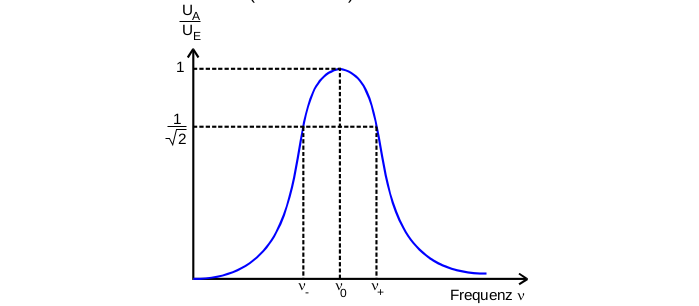
\includegraphics[width=\textwidth]{plots/Kaffeefilter.png}
        \caption{Die Gauß-verteilte Filterkurve eines Selektivverstärkers\cite{Versuchsanleitung}.}
        \label{fig:Kaffeefilter}
    \end{figure}

\subsection{Trivia}

    Die Materie-Proben liegen in Pulverform vor, welches sich in dünnen Glasröhrchen befindet. 
    Das Pulver hat hierbei eine geringere Dichte, als die gleiche Substanz hätte, wäre es ein Ein-Kristall.
    Deswegen wird eine effektiv wirkende Querschnittsfläche $Q_\text{eff}$ bei der Auswertung der Messdaten verwendet, 
    die umso kleiner ist, je dekrompimierter das Pulver der Probe ist. 
    Sie berechnet sich über 
    \begin{equation}
        Q_\text{eff}=Q\frac{\rho_\text{Pulver}}{\rho_\text{w}}=\frac{M_\text{Pulver}}{L \rho_\text{w}}
        \label{eqn:effQ}
    \end{equation}
    und wird mithilfe der Masse $M$ der Probe, der Länge $L$ der Probe (und somit die der Spule) und der 
    Dichte $\rho_\text{w}$ des Ein-Kristalls bestimmt. 